\documentclass{article}
\linespread{1.5}

\usepackage[utf8]{inputenc}
\usepackage{natbib}
\usepackage{graphicx}
\usepackage{authblk}
%For line number
\usepackage{lineno}

\title{Supplementary information\\ The Iron Law of Institutions: The co-evolution of institutions and hierarchy}
%\author{Cedric Perret$^1$, Emma Hart$^1$, Simon T. Powers$^1$}

\author[1]{Simon T.Powers}
\author[2]{Cedric Perret}
\author[2]{Thomas E. Currie}

\affil[1]{Edinburgh Napier University, Edinburgh EH10 5DT}
\affil[2]{University of Exeter, Penryn TR10 9Fr}
\date{In: Philosophical transactions of the Royal Society B\\
DOI: }


\begin{document}

\maketitle  

\begin{figure}, 
    \centering
    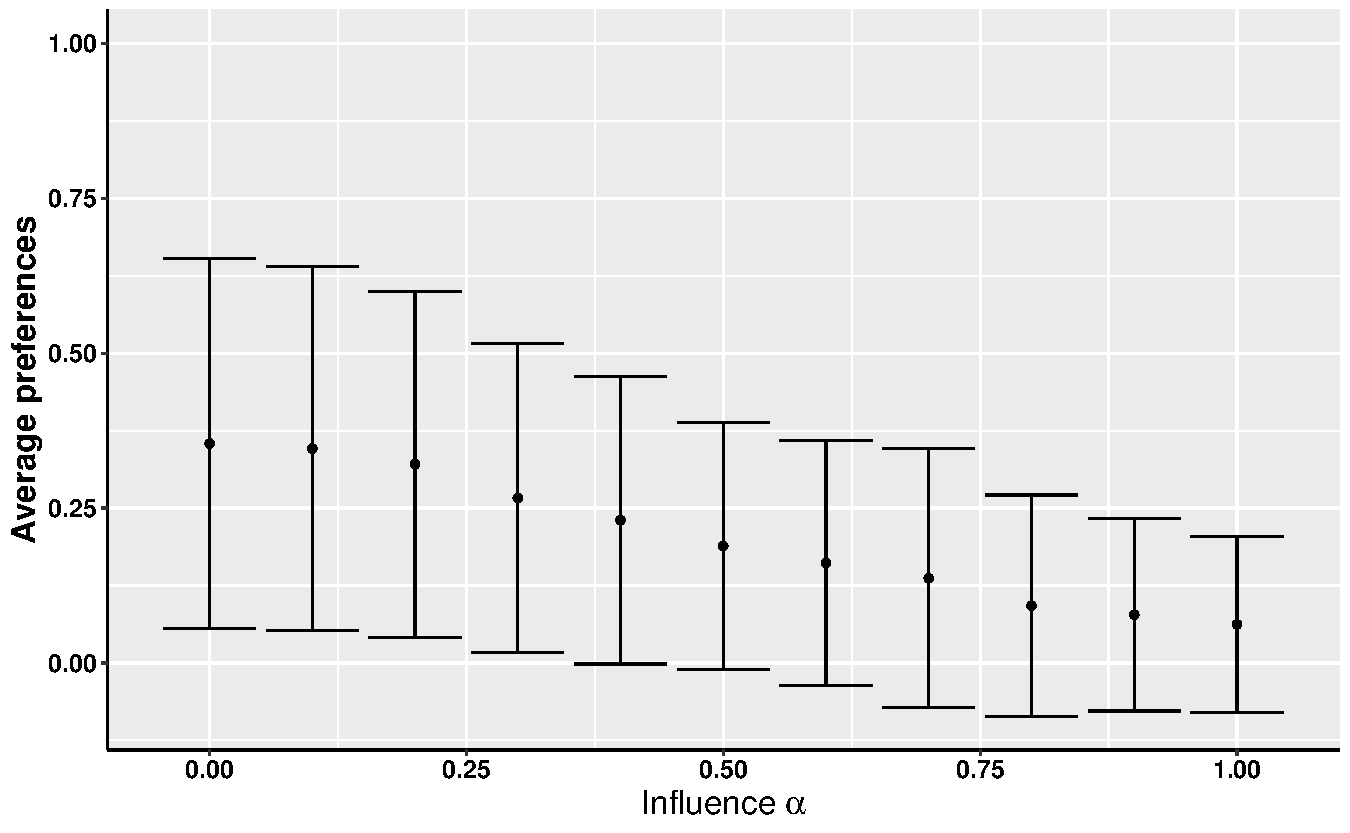
\includegraphics[width=1.2\linewidth]{Figures/pt_p_alpha.pdf}
    \caption{Average preferences as a function of influence $\alpha$. Error bars show the standard deviation}
    \label{figXThr}
\end{figure}


\begin{figure}, 
    \centering
    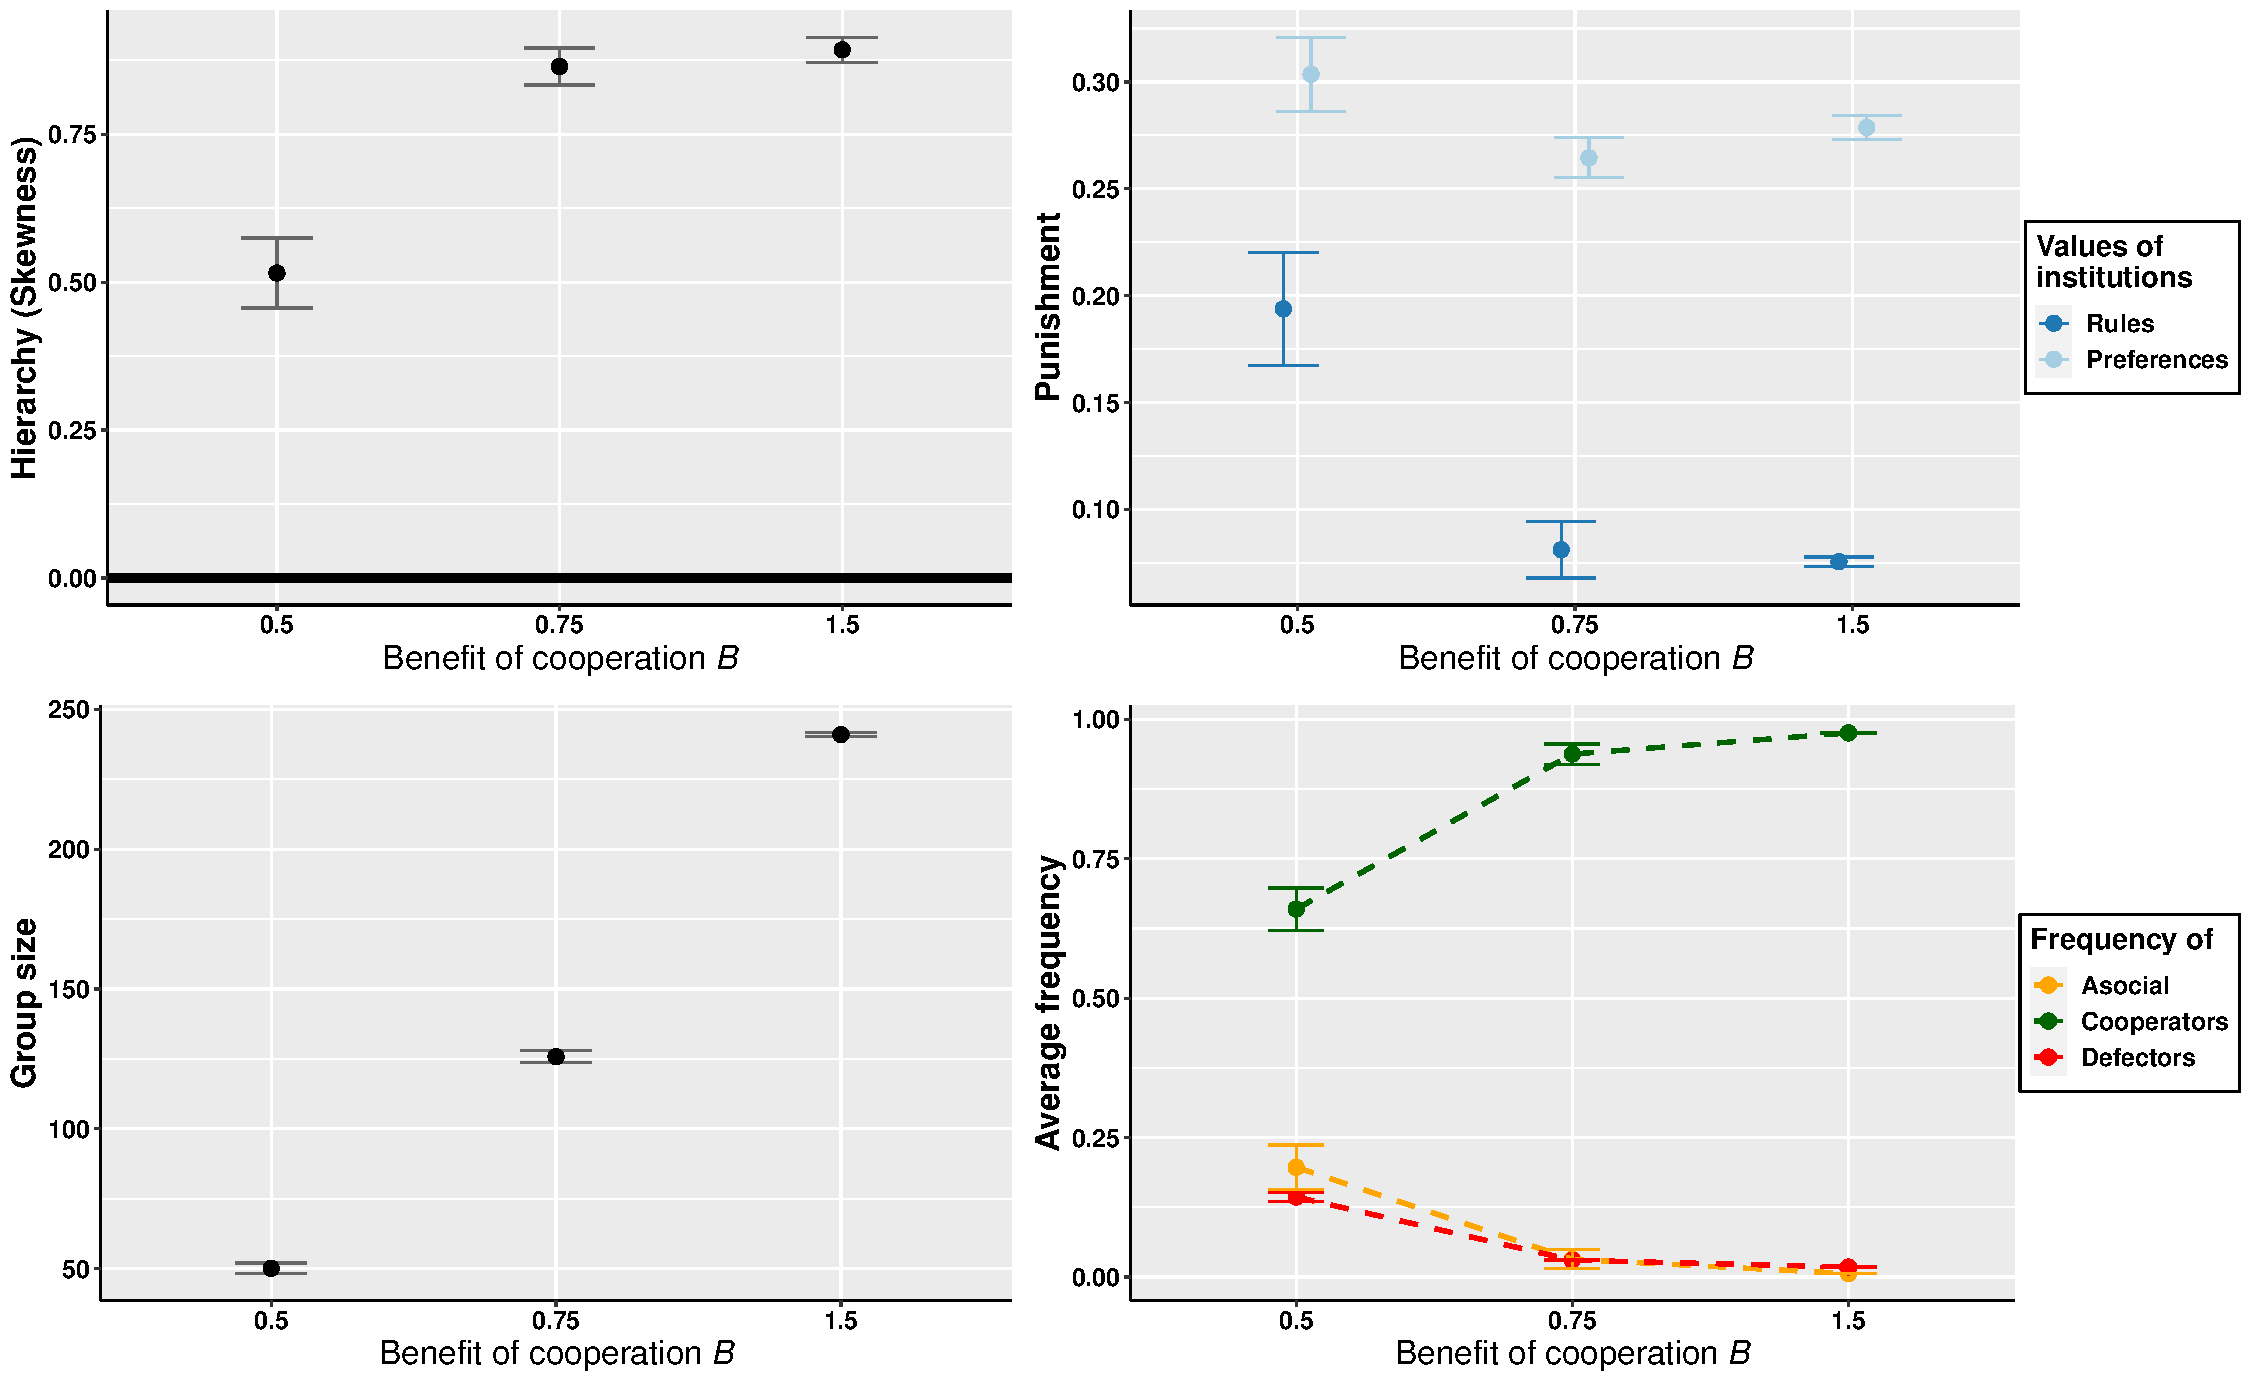
\includegraphics[width=1.2\linewidth]{Figures/pt_coopB_errorbar.pdf}
    \caption{The effect of varying the benefit of cooperation $B$. Error bars show the standard error across 10 replicates.}
    \label{figXThr}
\end{figure}



\end{document}